% Provenance (never printed): see sources/outline_sources.md (Year 2: ancient massifs,
% Caledonian and Variscan belts; the Wilson cycle; supercontinents). Caledonian phases after
% McKerrow, Mac Niocaill and Dewey (2000) and Schiffer et al. (2020); the Wilson cycle after
% Chenin et al. (2018) and Schiffer et al. (2020); the Variscan belt after Faure (2024);
% supercontinents after Nance (2022); Siccar Point after the IUGS Geoheritage description.
% Model ocean and supercontinent chart from figdata/bachelor-2/wilson.py. Exercise and problem
% values in the Book 4 scratch calculator calc/ch15.py.
\chapter{古老地块与威尔逊旋回}\label{ch:b2:wilson-cycle}

在苏格兰东南海岸的锡卡尔角，灰色砂岩层直立，
其上覆盖着一层向海缓倾的红色砂岩。这些灰色岩层形成于
志留纪早期的一个洋盆中，洋盆闭合时被褶皱并发育劈理；随后
它们被剥蚀成起伏不平的表面；晚泥盆世的红色砾石将其掩埋，而第二次
较为和缓的造山运动又使红层倾斜。一处悬崖记录了一个已经消失的洋
盆、一条已经消失的山带，以及接续其后的另一条山带。本章解读这类记录，
将其归纳为洋盆所遵循的旋回，并回溯到最长的节律，
即\omterm{def:b2:wilson-cycle:supercontinent}{超大陆}的聚合与裂解。
% ledger: iugs:siccar-orogenies, iugs:siccar-point

\begin{recall}
\textbf{来自中学分册}：泛大陆及其裂解、\omterm{def:b2:wilson-cycle:supercontinent}{超大陆}；不整合；
剥蚀速率、均衡回弹，以及被河流
侵蚀的山脉的指数衰减。\textbf{来自本科一年级分册}：大陆裂谷、被动大陆边缘和洋中脊、
全扩张速率与半扩张速率；俯冲与活动大陆边缘。
\textbf{来自\cref{ch:b2:crustal-melting}至\cref{ch:b2:himalaya-andes}}：\omterm{def:b2:crustal-melting:migmatite}{混合岩}与花岗岩；
\omterm{def:b2:alpine-orogen:orogen}{造山带}、\omterm{def:b2:alpine-orogen:ophiolite}{蛇绿岩}、缝合带、\omterm{def:b2:alpine-orogen:nappes}{推覆体}、\omterm{def:b2:alpine-orogen:foreland}{复理石}与\omterm{def:b2:alpine-orogen:foreland}{磨拉石}、\omterm{def:b2:alpine-orogen:foreland}{前陆盆地}；大陆碰撞与
\omterm{def:b2:himalaya-andes:types}{安第斯型造山带}；\omterm{def:b2:himalaya-andes:thickening}{地壳增厚}、艾里厚度与\omterm{def:b2:himalaya-andes:collapse}{重力垮塌}。
\end{recall}

\begin{omfigure}
\centering
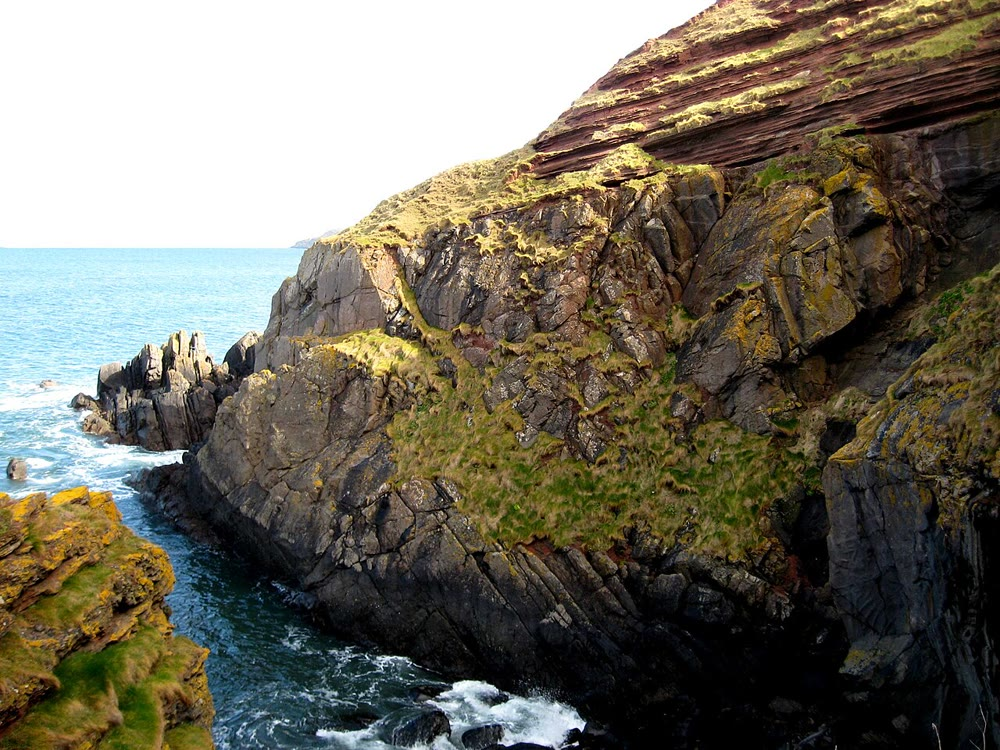
\includegraphics[width=0.64\linewidth]{images/book4/b2-15-siccar-point.jpg}
\par\smallskip{\small 锡卡尔角，角点东南侧：近直立的灰色
志留纪杂砂岩，在加里东造山运动中褶皱，位于
缓倾的上泥盆统红层之下。照片：dave souza, 2008, CC BY-SA 4.0。}
\end{omfigure}
% ledger: iugs:siccar-orogenies

\section{剥蚀至根部的山带}\label{sec:b2:wilson-cycle:old}

西欧与北美东部分布着若干远比阿尔卑斯山古老得多的
山带。它们的山峰已不复存在，但岩石犹存，此处讨论其中三条。

\emph{加里东}山带自挪威经苏格兰与爱尔兰延伸至纽芬兰及
阿巴拉契亚山北段，并继续穿越东格陵兰与斯瓦尔巴。它记录了一个
洋——伊阿珀托斯洋，它在早古生代位于西北方的劳伦古陆（
北美与格陵兰的前身）与东南及东侧的波罗的古陆和阿瓦隆尼亚之间。
其边缘约在 6 亿年前发生裂谷作用；其闭合自寒武纪
延续至泥盆纪，期间产生了一系列碰撞，使加里东造山运动
历时约 2 亿年。该名称指的是一处地域和一个洋，而不是一个时代。
% ledger: mckerrow00:caledonian, schiffer20:caledonides

\emph{瓦里斯坎}山带，旧文献称海西山带，横贯欧洲，自西南
英格兰、比利时经法国和伊比利亚延伸至中欧；\emph{阿巴拉契亚}山带与
北美东部的阿巴拉契亚山带互为孪生。二者共同记录了洋盆的闭合：
位于南方的冈瓦纳古陆与北方大陆之间的洋盆，后者刚刚
经加里东碰撞而拼合。它们的最后一次碰撞发生于晚石炭世和二叠纪，
留下了一条横穿南欧的东西向褶皱带，另一条呈东–西向，位于
北美东部与西北非之间，\omterm{def:b2:wilson-cycle:supercontinent}{超大陆}泛大陆随之形成。
% ledger: schiffer20:variscan, faure24:variscan

如何辨认一条已被侵蚀了 3 亿年的山带？
不能依靠地形，因其早已消失。应当寻找它的各组成部分，前几章
均已接触过这些部分：
\begin{itemize}
\item \emph{缝合带}，两侧或其间夹有\emph{\omterm{def:b2:alpine-orogen:ophiolite}{蛇绿岩}}，为闭合洋底的碎片；
\item 成带分布的\emph{变质岩}，多为高级变质，是增厚地壳的根部，
因上覆的千米岩层已被剥蚀，如今出露于地表；
\item \emph{花岗岩}与\emph{\omterm{def:b2:crustal-melting:migmatite}{混合岩}}，是增厚与升温所引起的地壳
熔融的产物；
\item 闭合洋盆与山带自身的沉积物：\emph{\omterm{def:b2:alpine-orogen:foreland}{复理石}}在汇聚过程中
堆积于深水盆地，\emph{\omterm{def:b2:alpine-orogen:foreland}{磨拉石}}堆积于\omterm{def:b2:alpine-orogen:foreland}{前陆盆地}与山间盆地；
\item \emph{角度不整合}，年轻岩层覆于先前已被褶皱并
剥蚀的岩层之上，由此可限定两者之间的变形时代。
\end{itemize}

\begin{definition}[准平原]\label{def:b2:wilson-cycle:peneplain}
称\emph{准平原}\index{准平原}为接近侵蚀基准面、起伏很小的陆地表面，
它由先前地貌经长期侵蚀，切穿硬度与结构各异的
岩石而成。
\end{definition}

瓦里斯坎山带是一条热\omterm{def:b2:alpine-orogen:orogen}{造山带}。在\cref{ch:b2:alpine-orogen}中的阿尔卑斯山，岩石
所遵循的变质梯度约为 \qty{8}{\celsius} 每千米；瓦里斯坎山带则
约为 \qty{30}{\celsius} 每千米。其地壳广泛熔融：法国中央地块与
阿莫里坎地块中，\omterm{def:b2:crustal-melting:migmatite}{混合岩}形成于约 3.3 亿至 3.25 亿年前，并
花岗岩侵入其中。这种熔融是其区别于西阿尔卑斯的主要特征。
碰撞结束后，增厚的地壳因伸展而减薄，变质岩
沿拆离带被带升，山间盆地随之张开；随后侵蚀将山链夷平为
二叠纪与三叠纪的\omterm{def:b2:wilson-cycle:peneplain}{准平原}，下一旋回的沉积物即堆积其上。
% ledger: faure24:variscan

\begin{omfigure}
\centering\small
\begin{tabular}{>{\raggedright\arraybackslash}p{0.2\linewidth}|>{\raggedright\arraybackslash}p{0.17\linewidth}|>{\raggedright\arraybackslash}p{0.52\linewidth}}
阶段 & 时代 & 碰撞对象 \\ \hline
佩诺布斯科特期 & 490--485 Ma & 岛弧逆冲至阿瓦隆尼亚边缘 \\
格兰皮安期、塔科尼克期 & 480--455 Ma & 岛弧与劳伦古陆相碰（苏格兰；阿巴拉契亚山北段） \\
谢尔维安期 & 晚奥陶世早期 & 阿瓦隆尼亚与波罗的古陆相碰；托恩奎斯特海闭合 \\
斯堪的纳维亚期 & 425--400 Ma & 波罗的古陆与劳伦古陆相碰；斯堪的纳维亚巨大\omterm{def:b2:alpine-orogen:nappes}{推覆体} \\
阿卡迪亚期 & 早泥盆世 & 来自冈瓦纳的\omterm{def:b2:wilson-cycle:terrane}{地体}与新拼合的大陆相碰；伊阿珀托斯洋闭合 \\
\end{tabular}
\par\smallskip{\small 加里东造山运动的主要阶段。早期阶段为
岛弧与岛弧或大陆的碰撞，晚期阶段为大陆之间的碰撞；多数
阶段在不同地点于不同时间开始。}
\end{omfigure}
% ledger: mckerrow00:phases, schiffer20:caledonides

上表所示的加里东造山阶段还显示了古老山带的另一特征：它们是复合体。在
两大陆相遇之前，岛弧与较小的地块相继而来，并被焊接其上。

\begin{definition}[地体；微大陆]\label{def:b2:wilson-cycle:terrane}
\emph{地体}\index{地体}是指一块被断层围限的地壳块体，其地质历史
与相邻地块不同，经板块运动被带到现今位置；它可以是
岛弧、大洋高原、洋底岩片或大陆碎片。
\emph{微大陆}\index{微大陆}是一块陆壳块体，
面积小于大陆，且与大陆之间以大洋地壳相隔。
\end{definition}

阿瓦隆尼亚就是这样一块地块：一条陆壳带离开冈瓦纳大陆边缘，
于奥陶纪在其身后张开 瑞克洋，穿越伊阿珀托斯洋，先与波罗的古陆
拼合，继而与劳伦古陆拼合。阿莫里卡和萨克索图林根随后相继加入，它们今分别位于法国和德国；
其缝合带以\omterm{def:b2:alpine-orogen:ophiolite}{蛇绿岩}为标志，将华力西\omterm{def:b2:alpine-orogen:orogen}{造山带}自老北方大陆中的北部前陆
至冈瓦纳中的南部前陆，划分为若干带。
% ledger: schiffer20:caledonides, schiffer20:variscan, faure24:variscan

\begin{omfigure}
\centering
\begin{tikzpicture}[x=0.5cm, y=0.5cm, font=\scriptsize]
\tikzset{cont/.style={fill=orange!25, draw=black!60, line width=0.4pt},
  terr/.style={fill=orange!45, draw=black!60, line width=0.4pt},
  ocn/.style={font=\scriptsize\itshape, text=blue!50!black},
  belt/.style={pattern=north east lines, pattern color=red!60!black, draw=red!60!black}}
% panel A
\begin{scope}
\fill[blue!6] (0,0) rectangle (9,8);
\draw[cont] (0.3,4.2) -- (3.0,4.0) -- (3.4,7.7) -- (0.3,7.7) -- cycle;
\node[align=center] at (1.7,6.0) {劳伦 \\古陆};
\draw[cont] (6.0,5.4) -- (8.7,5.0) -- (8.7,7.7) -- (6.4,7.7) -- cycle;
\node at (7.4,6.6) {波罗的古陆};
\draw[cont] (0.3,0.3) -- (8.7,0.3) -- (8.7,1.6) -- (0.3,1.9) -- cycle;
\node at (4.5,0.95) {冈瓦纳};
\draw[terr] (3.8,2.4) -- (6.6,2.2) -- (6.6,2.9) -- (3.8,3.1) -- cycle;
\node at (5.2,2.65) {阿瓦隆尼亚};
\node[ocn] at (4.6,5.4) {伊阿珀托斯洋};
\node[ocn] at (7.7,2.55) {瑞克洋};
\node[anchor=north west, font=\small\bfseries] at (0.1,8.9) {A：约 480 Ma};
\end{scope}
% panel B
\begin{scope}[xshift=5.0cm]
\fill[blue!6] (0,0) rectangle (9,8);
\draw[cont] (0.3,3.6) -- (3.0,3.4) -- (3.4,7.7) -- (0.3,7.7) -- cycle;
\draw[cont] (3.0,3.4) -- (3.4,7.7) -- (8.7,7.7) -- (8.7,4.4) -- (5.2,4.6) -- (5.0,3.4) -- cycle;
\draw[terr] (3.0,3.4) -- (5.0,3.4) -- (5.2,4.6) -- (8.7,4.4) -- (8.7,3.6) -- (3.0,2.8) -- cycle;
\draw[red!60!black, line width=1.2pt] (3.0,3.4) -- (3.4,7.7);
\draw[red!60!black, line width=1.2pt] (5.0,3.4) -- (5.2,4.6) -- (8.7,4.4);
\node[align=center] at (1.6,5.6) {劳伦 \\古陆};
\node at (6.6,5.7) {波罗的古陆};
\node at (6.4,3.75) {阿瓦隆尼亚};
\node at (6.0,7.1) {\textbf{劳亚古陆}};
\draw[cont] (0.3,0.3) -- (8.7,0.3) -- (8.7,1.3) -- (0.3,1.5) -- cycle;
\node at (4.5,0.8) {冈瓦纳};
\draw[terr] (2.2,1.9) -- (3.6,1.9) -- (3.6,2.3) -- (2.2,2.3) -- cycle;
\draw[terr] (5.0,1.8) -- (6.6,1.8) -- (6.6,2.2) -- (5.0,2.2) -- cycle;
\node[ocn] at (7.7,2.3) {瑞克洋};
\node[anchor=north west, font=\small\bfseries] at (0.1,8.9) {B：约 420 Ma};
\end{scope}
% panel C
\begin{scope}[xshift=10.0cm]
\fill[blue!6] (0,0) rectangle (9,8);
\draw[cont] (0.3,3.0) -- (8.7,3.0) -- (8.7,7.7) -- (0.3,7.7) -- cycle;
\draw[cont] (0.3,0.3) -- (8.7,0.3) -- (8.7,3.0) -- (0.3,3.0) -- cycle;
\fill[belt] (0.3,2.5) -- (8.7,2.5) -- (8.7,3.5) -- (0.3,3.5) -- cycle;
\node[fill=orange!25, inner sep=1pt] at (4.5,5.6) {劳亚古陆};
\node[fill=orange!25, inner sep=1pt] at (4.5,1.3) {冈瓦纳};
\node[fill=white, fill opacity=0.85, text opacity=1, inner sep=1pt, align=center] at (4.5,3.0)
  {华力西–阿巴拉契亚造山带};
\node[ocn] at (7.6,0.7) {};
\node[anchor=north west, font=\small\bfseries] at (0.1,8.9) {C：约 300 Ma，泛大陆};
\end{scope}
\end{tikzpicture}
\par\smallskip{\small 伊阿珀托斯洋与 瑞克洋闭合的三个时刻，以示意草图表示，
不含地图投影，也不含比例尺：位置、大小和形状仅具拓扑意义。
A：阿瓦隆尼亚已离开冈瓦纳，其身后张开 瑞克洋。B：伊阿珀托斯洋已闭合；
劳伦、波罗的与阿瓦隆尼亚沿加里东缝合带（红线）拼合为劳亚古陆；
较小地块正穿越 瑞克洋。C：冈瓦纳已与劳亚古陆沿
华力西–阿巴拉契亚\omterm{def:b2:alpine-orogen:orogen}{造山带}（斜线阴影）拼合。}
\end{omfigure}
% ledger: mckerrow00:caledonian, mckerrow00:phases, schiffer20:caledonides, schiffer20:variscan, faure24:variscan

\section{威尔逊旋回}\label{sec:b2:wilson-cycle:cycle}

1966 年，威尔逊提出疑问：大西洋是否曾闭合，随后
又重新张开？古生代早、中期的化石告诉他，当时曾有一个宽阔的大洋
将北美与西欧的动物群隔开的这一大洋，自晚古生代至中生代中期
已不复存在。现代大西洋张开的位置，几乎正是那个古老大洋
即伊阿珀托斯洋闭合的位置。
% ledger: schiffer20:wilson, chenin18:cycle

\begin{definition}[威尔逊旋回]\label{def:b2:wilson-cycle:wilson}
\emph{威尔逊旋回}\index{威尔逊旋回}是指大洋盆地在大陆边缘之间张开并再次闭合所经历的
一系列阶段：大陆裂谷作用，
破裂与海底扩张，伴有被动大陆边缘的大洋扩张，俯冲的开始，
大洋的收窄与闭合，大陆碰撞，以及
\omterm{def:b2:alpine-orogen:orogen}{造山带}的垮塌与侵蚀，此后拼合的大陆可能沿同一地带再次裂开。
\end{definition}

下图按上述阶段展示。它们是前面各章内容的有序排列：
本科一年级分册中的裂谷与被动大陆边缘、活动大陆边缘及其火山弧、
阿尔卑斯与喜马拉雅的碰撞、西藏的\omterm{def:b2:himalaya-andes:collapse}{重力垮塌}，以及
古老\omterm{def:b2:alpine-orogen:orogen}{造山带}的缓慢剥蚀。

\begin{omfigure}
\centering
\begin{tikzpicture}[x=0.38cm, y=0.38cm, font=\scriptsize]
\tikzset{crust/.style={fill=orange!25, draw=black!60, line width=0.3pt},
  ocrust/.style={fill=gray!45, draw=black!60, line width=0.3pt},
  sea/.style={fill=blue!8},
  ttl/.style={anchor=west, font=\scriptsize\bfseries}}
% 1 continent
\begin{scope}
\draw[crust] (0,0) -- (16,0) -- (16,2) -- (0,2) -- cycle;
\node[ttl] at (0,3.1) {1\enspace 一块大陆};
\end{scope}
% 2 rift
\begin{scope}[xshift=7.2cm]
\draw[crust] (0,0) -- (7,0) -- (7,2) -- (6.2,2) -- (5.4,1.0) -- (0,2) -- cycle;
\draw[crust] (9,0) -- (16,0) -- (16,2) -- (10.6,1.0) -- (9.8,2) -- (9,2) -- cycle;
\fill[red!50] (7,0) -- (9,0) -- (8.6,1.2) -- (7.4,1.2) -- cycle;
\draw[thick] (6.2,2) -- (7,0.4); \draw[thick] (9.8,2) -- (9,0.4);
\node[ttl] at (0,3.1) {2\enspace 裂谷};
\end{scope}
% 3 young ocean
\begin{scope}[yshift=-2.4cm]
\fill[sea] (5,2) -- (11,2) -- (11,0.6) -- (5,0.6) -- cycle;
\draw[crust] (0,0) -- (5,0) -- (6.2,0.5) -- (5,2) -- (0,2) -- cycle;
\draw[crust] (16,0) -- (11,0) -- (9.8,0.5) -- (11,2) -- (16,2) -- cycle;
\draw[ocrust] (6.2,0.5) -- (9.8,0.5) -- (9.8,0) -- (6.2,0) -- cycle;
\draw[red!70!black, thick] (8,0.5) -- (8,1.0);
\node[ttl] at (0,3.1) {3\enspace 新生大洋};
\end{scope}
% 4 wide ocean
\begin{scope}[xshift=7.2cm, yshift=-2.4cm]
\fill[sea] (2.5,2) -- (13.5,2) -- (13.5,0.4) -- (2.5,0.4) -- cycle;
\draw[crust] (0,0) -- (2.5,0) -- (3.4,0.4) -- (2.5,2) -- (0,2) -- cycle;
\draw[crust] (16,0) -- (13.5,0) -- (12.6,0.4) -- (13.5,2) -- (16,2) -- cycle;
\draw[ocrust] (3.4,0.4) -- (12.6,0.4) -- (12.6,-0.4) -- (3.4,-0.4) -- cycle;
\draw[red!70!black, thick] (8,0.4) -- (8,0.9);
\node[anchor=north] at (3,-0.1) {被动边缘};
\node[anchor=north] at (13,-0.1) {被动边缘};
\node[ttl] at (0,3.1) {4\enspace 宽阔大洋};
\end{scope}
% 5 subduction begins
\begin{scope}[yshift=-4.8cm]
\fill[sea] (2.5,2) -- (13.5,2) -- (13.5,0.4) -- (2.5,0.4) -- cycle;
\draw[crust] (0,0) -- (2.5,0) -- (3.4,0.4) -- (2.5,2) -- (0,2) -- cycle;
\draw[crust] (16,-0.4) -- (13.3,-0.4) -- (12.6,0.4) -- (13.5,2) -- (16,2) -- cycle;
\draw[ocrust] (3.4,0.4) -- (12.6,0.4) -- (11.6,-1.6) -- (3.4,-0.4) -- cycle;
\fill[red!60!black] (14.2,2) -- (14.6,2.7) -- (15.0,2) -- cycle;
\draw[red!70!black, thick] (7,0.4) -- (7,0.9);
\node[anchor=north] at (13.5,-0.5) {海沟};
\node[ttl] at (0,3.1) {5\enspace 俯冲开始};
\end{scope}
% 6 ocean closes
\begin{scope}[xshift=7.2cm, yshift=-4.8cm]
\fill[sea] (5.5,2) -- (10.5,2) -- (10.5,0.4) -- (5.5,0.4) -- cycle;
\draw[crust] (0,0) -- (5.5,0) -- (6.4,0.4) -- (5.5,2) -- (0,2) -- cycle;
\draw[crust] (16,-0.4) -- (11.3,-0.4) -- (10.6,0.4) -- (11.5,2.4) -- (16,2.4) -- cycle;
\draw[ocrust] (6.4,0.4) -- (10.6,0.4) -- (9.4,-1.8) -- (6.4,-0.4) -- cycle;
\fill[red!60!black] (12.4,2.4) -- (12.8,3.1) -- (13.2,2.4) -- cycle;
\node[anchor=north west] at (11.6,-0.5) {岛弧、海沟};
\node[ttl] at (0,3.1) {6\enspace 大洋闭合};
\end{scope}
% 7 collision
\begin{scope}[yshift=-7.2cm]
\draw[crust] (0,0) -- (16,0) -- (16,2) -- (10,2) -- (8.6,3.6) -- (7.4,3.4) -- (6,2) -- (0,2) -- cycle;
\fill[crust] (5.6,0) -- (10.4,0) -- (9.6,-1.6) -- (6.4,-1.6) -- cycle;
\draw[black!60, line width=0.3pt] (5.6,0) -- (6.4,-1.6) -- (9.6,-1.6) -- (10.4,0);
\draw[red!60!black, line width=1pt] (8.6,3.6) -- (7.6,-1.6);
\node[anchor=west, text=red!60!black] at (9.0,3.5) {缝合带};
\node[ttl] at (0,3.1) {7\enspace 碰撞};
\end{scope}
% 8 worn flat
\begin{scope}[xshift=7.2cm, yshift=-7.2cm]
\draw[crust] (0,0) -- (16,0) -- (16,2) -- (0,2) -- cycle;
\draw[red!60!black, line width=1pt] (8.4,2) -- (7.6,0);
\fill[pink!60!red!40] (6.0,1.0) ellipse (0.7 and 0.4);
\node[anchor=north] at (8,-0.1) {老根之上的准平原};
\node[ttl] at (0,3.1) {8\enspace 造山带夷平后或再裂开};
\end{scope}
\end{tikzpicture}
\par\smallskip{\small \omterm{def:b2:wilson-cycle:wilson}{威尔逊旋回}各阶段的示意剖面（未按比例）：
橙色为陆壳，灰色为洋壳，红色为洋脊，火山弧的火山以三角形表示；
末幅中，缝合带与花岗岩仍处于正常厚度的地壳之中。}
\end{omfigure}
% ledger: chenin18:cycle, schiffer20:wilson

\subsection{有多宽，有多长？}

海洋在洋脊处通过海底扩张而扩大，在海沟处通过俯冲而缩小。
简单的核算即可给出其宽度。

\begin{proposition}[一个旋回中海洋的宽度]\label{prop:b2:wilson-cycle:width}
设海洋在时刻 $t_0$ 张开，并以其洋脊的全扩张速率 $V_s$ 扩大，直至
某一边缘在时刻 $t_1$ 开始形成俯冲带，并以速率 $V_c$ 消耗洋底
（相对该边缘），其中 $V_c > V_s$，洋脊仍在扩张。宽度为
\[
  W(t) = V_s\,(t - t_0) \quad (t_0 \le t \le t_1), \qquad
  W(t) = V_s\,(t_1 - t_0) - (V_c - V_s)\,(t - t_1) \quad (t \ge t_1),
\]
在 $t_1$ 时最大，海洋闭合所需时间为 $V_s(t_1 - t_0)/(V_c - V_s)$
，自俯冲开始算起。若扩张对称，洋脊朝海沟以 $V_c - V_s/2$ 的速度移动。
\end{proposition}

\begin{proof}
固定海沟所在的边缘。在 $t_1$ 之前，两侧边缘以全
扩张速率 $V_s$ 分离，宽度以 $V_s$ 由零增长。$t_1$ 之后，海沟与洋脊之间的板块
朝海沟以 $V_c$ 运动；洋脊使该板块与远侧板块之间的距离增加 $V_s$，
故远侧边缘朝海沟的运动速率为 $V_c - V_s$，
即宽度减小的速率。宽度经过 $V_s(t_1 - t_0)/(V_c -
V_s)$ 后降为零。若扩张对称，洋脊的速度为其两侧板块速度的平均值，
即 $(V_c + (V_c - V_s))/2 = V_c - V_s/2$。
\end{proof}

下图针对一个伊阿珀托斯型模型海洋演示了这一核算，其扩张始于
\qty{570}{Ma}起，速率为每年 \qty{30}{mm}，俯冲始于 \qty{490}{Ma}，每年消耗
\qty{60}{mm}。这些速率为假设，是今日海洋中测得尺度的整数取值；真实的
伊阿珀托斯洋既不如此简单，也不如此为人所熟知。模型海洋宽达 \qty{2400}{km}，
并闭合于 \qty{410}{Ma}，处于斯堪的纳维亚碰撞的时间跨度之内。
% values (wilson.py): max_width_km 2400, closure_Ma 410; ledger: mckerrow00:caledonian, schiffer20:caledonides

\begin{omfigure}
\centering
% figdata/bachelor-2/wilson.py part ocean (model values: assumptions)
\begin{tikzpicture}
\begin{axis}[width=0.8\linewidth, height=5.0cm, x dir=reverse, xmin=360, xmax=600, ymin=0,
  ymax=3300, ytick={0,1000,2000,3000}, xlabel={年龄（\unit{Ma}）}, ylabel={海洋宽度（\unit{km}）},
  tick label style={font=\scriptsize}, label style={font=\small}, xtick={600,560,...,360}]
\addplot[omThm, line width=1.2pt] table[x=t_Ma, y=width_km] {figdata/out/bachelor-2-wilson-ocean.dat};
\draw[dashed, black!50] (axis cs:490,0) -- (axis cs:490,2400);
\draw[dashed, black!50] (axis cs:570,0) -- (axis cs:570,2750);
\draw[dashed, black!50] (axis cs:410,0) -- (axis cs:410,2750);
\node[font=\scriptsize, anchor=south] at (axis cs:570,2750) {开始扩张};
\node[font=\scriptsize, anchor=south west] at (axis cs:488,2400) {俯冲开始};
\node[font=\scriptsize, anchor=south] at (axis cs:410,2750) {碰撞};
\node[font=\scriptsize, anchor=west] at (axis cs:540,600) {以 $V_s$ 张开};
\node[font=\scriptsize, anchor=south west, align=left] at (axis cs:446,1150) {闭合 \\速率 $V_c - V_s$};
\end{axis}
\end{tikzpicture}
\par\smallskip{\small 一个\omterm{def:b2:wilson-cycle:wilson}{威尔逊旋回}中模型海洋的宽度，由
\cref{prop:b2:wilson-cycle:width}给出，取 $V_s = \qty{30}{mm}$ 每年，自 \qty{570}{Ma} 起，与 $V_c
= \qty{60}{mm}$ 每年，自 \qty{490}{Ma} 起。时间自左向右推进。}
\end{omfigure}

\subsection{在闭合处重新张开}

威尔逊的想法建立在一个力学观点之上：古老\omterm{def:b2:alpine-orogen:orogen}{造山带}是薄弱带，而被拉开的大陆
倾向于沿其薄弱带破裂，而不是穿过其坚固、稳定的
内部。

\begin{definition}[构造活化]\label{def:b2:wilson-cycle:reactivation}
称既有构造的\emph{构造活化}\index{构造活化}，
即既有构造（断层、剪切带、缝合带、岩性接触面）上变形的重新集中，
其发生于可能不同于该构造形成时的后期应力场之下。
\end{definition}

北大西洋是这一检验的实例，而它只部分符合。在中大西洋
年轻的洋盆紧随阿巴拉契亚山脉。在斯堪的纳维亚与格陵兰之间，裂解
大体沿加里东\omterm{def:b2:alpine-orogen:orogen}{造山带}展布。更南部则不然：伊阿珀托斯缝合带仍穿过
英格兰北部与爱尔兰中部，而大西洋在其西侧张开，留下
劳伦古陆古老地壳的碎片残留于欧洲西北缘，围绕罗卡尔与哈顿分布。
更西北处，拉布拉多海与巴芬湾直接横切较老的克拉通和
\omterm{def:b2:alpine-orogen:orogen}{造山带}。古老构造会引导后期裂谷，但并非总是如此：一处薄弱带若已冷却超过
3000 万至 5000 万年，可能已变强，而新裂谷可能沿地幔中更深层的
构造延伸，而不是沿地壳缝合带。\omterm{def:b2:wilson-cycle:wilson}{威尔逊旋回}是指南，而非定律。
% ledger: schiffer20:wilson, schiffer20:reactivation

并非每个旋回都会张开宽阔的洋盆。许多\omterm{def:b2:alpine-orogen:orogen}{造山带}闭合的是初生洋盆，即刚开始
扩张、宽度小于约 \qty{500}{km} 的裂谷，如阿尔卑斯山、比利牛斯山以及
西欧的华力西带大部分。另一些则闭合宽阔、成熟的洋盆，如斯堪的纳维亚
加里东\omterm{def:b2:alpine-orogen:orogen}{造山带}。差别在末期显现：闭合宽阔洋盆的\omterm{def:b2:alpine-orogen:orogen}{造山带}带有长寿命的岛弧，
该岛弧抽取了其下方地幔的可熔组分，因而垮塌时\omterm{def:b2:magma-emplacement:magma}{岩浆}匮乏，
如加里东\omterm{def:b2:alpine-orogen:orogen}{造山带}。闭合狭窄盆地的\omterm{def:b2:alpine-orogen:orogen}{造山带}位于\omterm{def:b2:mantle-melting:fertility}{饱满地幔}之上，其
垮塌可以富含\omterm{def:b2:magma-emplacement:magma}{岩浆}，如华力西带，那里莫霍面现已平坦，
下地壳呈层状，可解读为地壳之下底侵的玄武岩，或是
在高温时被剪切的下地壳。在几千万年之内，\omterm{def:b2:alpine-orogen:orogen}{造山带}的热
异常消退，其构造则保留下来。
% ledger: chenin18:cycle

\section{超大陆}\label{sec:b2:wilson-cycle:supercontinents}

\begin{definition}[超大陆；超大陆旋回]\label{def:b2:wilson-cycle:supercontinent}
称\emph{超大陆}\index{超大陆}为汇聚了地球大部分
大陆地壳于单一块体中的陆块。\emph{超大陆旋回}\index{超大陆旋回}
是大陆阶段性地聚合为一个超大陆、随后再裂解的
过程，并在地球历史中反复出现。
\end{definition}

泛大陆由魏格纳重建、中学分册也有描述，约存在于 3.25 亿
年前至 2 亿年前。更早的\omterm{def:b2:wilson-cycle:supercontinent}{超大陆}曾被提出：泛努提亚约 6.2 亿至
5.8 亿年前，其存在仍有争议；罗迪尼亚约 9.5 亿至 8 亿年前；
努纳，又称哥伦比亚，约 16 亿至 14 亿年前；更不确定的还有肯诺兰
古陆约 27 亿至 25 亿年前，以及乌尔约 30 亿年前。它们似乎
每隔约 5 亿年聚合并裂解一次，大约自太古宙晚期
以来。该旋回已与造山时代、花岗岩的年龄峰值
及其所含锆石颗粒的年龄峰值、地壳增长、大火成岩省相联系，
也与海平面和气候相联系：\omterm{def:b2:wilson-cycle:supercontinent}{超大陆}的聚合往往与
降温同时发生。
% ledger: nance22:supercontinents

\begin{omfigure}
\centering
% figdata/bachelor-2/wilson.py part supercontinents; ledger: nance22:supercontinents
\begin{tikzpicture}
\begin{axis}[width=0.86\linewidth, height=4.6cm, x dir=reverse, xmin=0, xmax=3300, ymin=-0.7,
  ymax=6.5, ytick=\empty, xlabel={年龄 (\unit{Ma})}, tick label style={font=\scriptsize},
  label style={font=\small}, xtick={0,500,...,3000}, axis y line*=left,
]
\addplot[only marks, mark=*, mark size=1.6pt, omThm,
  error bars/.cd, x dir=both, x explicit, error bar style={line width=3pt, omThm!60}, error mark=none]
  table[x=mid_Ma, y=row, x error=half_Ma] {figdata/out/bachelor-2-wilson-supercontinents.dat};
\node[font=\scriptsize, anchor=south, yshift=1pt, text=omThm] at (axis cs:3000,0) {乌尔};
\node[font=\scriptsize, anchor=south, yshift=1pt, text=omThm] at (axis cs:2600,1) {肯诺兰};
\node[font=\scriptsize, anchor=south, yshift=1pt, text=omThm] at (axis cs:1500,2) {努纳--哥伦比亚};
\node[font=\scriptsize, anchor=south, yshift=1pt, text=omThm] at (axis cs:875,3) {罗迪尼亚};
\node[font=\scriptsize, anchor=south, yshift=1pt, text=omThm] at (axis cs:600,4) {潘诺西亚};
\node[font=\scriptsize, anchor=south, yshift=1pt, text=omThm] at (axis cs:262.5,5) {泛大陆};
\end{axis}
\end{tikzpicture}
\par\smallskip{\small 地球历史上的\omterm{def:b2:wilson-cycle:supercontinent}{超大陆}，自聚合至解体，依据近期一篇综述所定年代：
条带表示所引区间（乌尔仅为一个估计值），
圆点表示各区间的中点。泛努提亚、肯诺兰古陆与乌尔仍有争议。时间自左向右推移。}
\end{omfigure}

该旋回真的具有周期性吗？图中各区间中点之间相隔
400、1100、625、275 和 337.5 百万年：平均约 550，但差异可达四倍之多。
“大约半个十亿年”只是一种趋势，而非时钟，况且更早的
\omterm{def:b2:wilson-cycle:supercontinent}{超大陆}所依据的证据稀少。
% values (wilson.py): spacings 400 1100 625 275 337.5, mean 547.5 Myr

\section{从山脉到平原}\label{sec:b2:wilson-cycle:erosion}

是什么使喜马拉雅这样的山脉变成布列塔尼的低矮丘陵？高中分册
建立了一个模型：河流以正比于平均海拔 $kh$ 的速率剥蚀山脉，
而从山顶移去的每一米都会因均衡回弹而部分回返，因此只有
比例为 $f = (\rho_m - \rho_c)/\rho_m$ 的部分以高度的形式损失。平均海拔此后
按下式衰减：
\[
  h(t) = h_0\,e^{-k f t} ,
\]
时间常数为 $\tau = 1/(kf)$。在大型中纬度盆地中，剥蚀速率与平均地形起伏成正比，
若无隆升，地形起伏降至原值的十分之一所需时间约为 1100 万年：
$k = \ln 10/11 \approx 0.21$ 每百万年。取密度
2700 与 \qty{3300}{kg.m^{-3}}，则 $f = 0.18$，$\tau \approx \qty{26}{Ma}$：一座高 \qty{3}{km} 的山脉，
约 3000 万年后仍高 \qty{1}{km}，约 6000 万年后则降至
\qty{300}{m} 以下。
% ledger: ahnert70:decay; values (wilson.py): k 0.20933 /Myr, f 0.18182, tau 26.275 Myr

同一种回弹也解释了古老\omterm{def:b2:alpine-orogen:orogen}{造山带}为何会暴露其根部。要使由 $H$ 增厚到 $T$ 的地壳
回到海平面，必须剥蚀掉全部额外厚度 $T - H$，而平均海拔仅为
$(T - H)f$：被移去的岩石约为山脉高度的 5.5 倍。原本位于 20 或 \qty{30}{km} 深处
的根部岩石出露地表：老地块中的\omterm{def:b2:crustal-melting:migmatite}{混合岩}、花岗岩与高级片麻岩，
例如法国
中央高原地块的那些岩石。
% ledger: ahnert70:decay

瓦里斯坎\omterm{def:b2:alpine-orogen:orogen}{造山带}的最后一次碰撞结束于约 2.9 亿年前，
其后在二叠纪与三叠纪期间被夷平为\omterm{def:b2:wilson-cycle:peneplain}{准平原}，时间约为模型所给的 6000 万年左右。
坍塌可以加快这一过程：增厚地壳的伸展，如今日的西藏，会直接使其减薄，
无需等待河流。而在锡卡尔角，晚泥盆世的砾岩覆盖在
志留纪的岩层之上，这些岩层在加里东碰撞中被褶皱，其下的古老地表
在硬层与软层之间仍保留着一定起伏。
% ledger: faure24:variscan, iugs:siccar-orogenies

\begin{inthefield}[读懂角度不整合]
研究锡卡尔角一类角度不整合的地质学家，首先在许多地点测量界面上下
岩层的产状，即走向与倾角。他们依据递变层理或岩层底面的痕迹，
判断下层岩层的顶底方向，因为褶皱岩层可能已经倒转。他们再考察界面本身：
其地形起伏、其下的风化层，以及其上砾岩中老岩石的卵石。随后测定年代：
下方最年轻的化石给出褶皱不可能发生之前的年龄，上方最古老的化石
给出此前褶皱已经发生、陆地已被剥蚀的年龄。两个界线之间的时间间隔即为造山运动。
在锡卡尔角，下层岩层为早志留世，上层岩层为晚泥盆世，
加里东褶皱、隆升与剥蚀恰好落在两者之间；
上层岩层平缓的倾斜则更为年轻，
属于瓦里斯坎期。
\end{inthefield}
% ledger: iugs:siccar-orogenies, ics:base.Silurian, ics:base.Devonian, ics:base.Carboniferous

\section*{练习}\label{sec:b2:wilson-cycle:exercises}

练习数据：$g = \qty{9.8}{m.s^{-2}}$；地壳与地幔的密度分别为
\qty{2700}{kg.m^{-3}} 和 \qty{3300}{kg.m^{-3}}；正常地壳 $H = \qty{35}{km}$；志留纪、泥盆纪与石炭纪底界的年龄分别为
443.1、419.6 和 \qty{358.9}{Ma}，三叠纪底界的年龄为
\qty{251.9}{Ma}。

\begin{exercise}[$\star$]\label{exo:b2:wilson-cycle:1}
伊阿珀托斯洋的边缘约在 \qty{600}{Ma} 开始裂开；主要的加里东碰撞，即
斯堪的纳维亚期，约在 \qty{400}{Ma} 结束；与劳伦古陆的首次弧－陆碰撞约在
\qty{480}{Ma} 开始。(a) 伊阿珀托斯洋的整个旋回持续了多久？(b) 碰撞持续了多久？
(c) 为什么“加里东”不应用来表示一个年代？
\end{exercise}

\begin{exercise}[$\star$]\label{exo:b2:wilson-cycle:2}
将下列情形按\omterm{def:b2:wilson-cycle:wilson}{威尔逊旋回}的顺序排列，并说明每一情形所处的阶段：(a) 红海，一个介于年轻裂谷边缘之间的狭窄洋盆；(b) 喜马拉雅；(c) 东非裂谷；
(d) 大西洋，宽阔，两侧均为被动大陆边缘；(e) 南美洲的太平洋边缘；
(f) 建在古老花岗岩与片麻\omterm{def:b2:magma-emplacement:bodies}{岩基}底之上的布列塔尼低矮丘陵。
求将下列情形按\omterm{def:b2:wilson-cycle:wilson}{威尔逊旋回}的顺序排列，并说明每一情形所处的阶段
\end{exercise}

\begin{exercise}[$\star$]\label{exo:b2:wilson-cycle:3}
在锡卡尔角，早志留世的岩层位于晚泥盆世岩层之下。(a) 依据上述数据，
褶皱、隆升与剥蚀必须发生在哪两个界线之间？(b) 它们最长可能持续多久？
(c) 按顺序列出悬崖所记录的事件。
\end{exercise}

\begin{exercise}[$\star$]\label{exo:b2:wilson-cycle:4}
判断下列各项是\omterm{def:b2:wilson-cycle:terrane}{地体}、\omterm{def:b2:wilson-cycle:terrane}{微大陆}、两者兼是还是两者都不是，并说明理由：(a) 阿瓦隆尼亚；
(b) 劳伦古陆；(c) 增生到大陆上的岛弧；(d) 伊阿珀托斯缝合带。
\end{exercise}

\begin{exercise}[$\star\star$]\label{exo:b2:wilson-cycle:5}
取\omterm{def:b2:wilson-cycle:supercontinent}{超大陆}乌尔（3000）、肯诺兰古陆（2600）、
努纳（1500）、罗迪尼亚（875）、泛努提亚（600）与泛大陆（262.5）的区间中点，单位为百万年前。
(a) 计算这五个间隔及其平均值。(b) 最大间隔与最小间隔之比是多少？
(c) 去掉存疑的肯诺兰古陆与乌尔，其余四个的平均间隔是多少？
“大约半个十亿年”是一个周期吗？
\end{exercise}

\begin{exercise}[$\star\star$]\label{exo:b2:wilson-cycle:6}
一个宽 \qty{3000}{km} 的大洋，在一侧边缘以每年 \qty{70}{mm} 的速率开始俯冲，
同时其洋脊以每年 \qty{25}{mm} 的速率扩张。(a) 它需要多长时间闭合？
(b) 若扩张立即停止，需要多长时间？(c) 洋脊被俯冲之后，
由哪个板块的运动决定闭合速率？
\end{exercise}

\begin{exercise}[$\star\star$]\label{exo:b2:wilson-cycle:7}
设地壳熔融约在 \qty{700}{\celsius} 开始，地表温度为
\qty{0}{\celsius}。(a) 沿梯度
每千米 \qty{8}{\celsius} 时，该温度在何深度达到？每千米 \qty{30}{\celsius} 时呢？(b) 下列哪条\omterm{def:b2:alpine-orogen:orogen}{造山带}，
阿尔卑斯\omterm{def:b2:alpine-orogen:orogen}{造山带}还是海西\omterm{def:b2:alpine-orogen:orogen}{造山带}，应当出露地壳成因的\omterm{def:b2:crustal-melting:migmatite}{混合岩}和花岗岩？
(c) 在第一种情形中，为何固定梯度会高估深度？
\end{exercise}

\begin{exercise}[$\star\star$]\label{exo:b2:wilson-cycle:8}
海西期碰撞约于 \qty{290}{Ma} 结束，至二叠纪与
三叠纪，\omterm{def:b2:wilson-cycle:peneplain}{准平原}已形成。取本章衰减模型，$\tau = \qty{26.3}{Ma}$。(a) 一座山脉
从平均海拔 \qty{3}{km} 降至 \qty{0.3}{km} 需多长时间？(b) 那将对应于
什么年龄？(c) 要在三叠纪底界前降至该高度，时间常数应为多少？
(d) 何种过程能缩短这一时间？
\end{exercise}

\begin{exercise}[$\star\star$]\label{exo:b2:wilson-cycle:9}
(a) 试解释为何英格兰北部和爱尔兰中部的伊阿珀托斯缝合带，以及
罗卡尔附近的劳伦古陆地壳，说明大西洋并未严格沿古老缝合带重新张开。
(b) 地质学家应当预期在缝合带两侧的古老基底中发现什么？
在爱尔兰？(c) 阿巴拉契亚山脉直至早二叠世仍在变形，裂谷作用
在造山运动之后约 8000 万年开始。试与 3000 至 5000 万年相比，
此后冷却带可能过于坚固而无法再活化。
\end{exercise}

\begin{exercise}[$\star\star\star$]\label{exo:b2:wilson-cycle:10}
一个宽 \qty{3000}{km} 的大洋，洋脊位于其中部，距离一条海沟 \qty{1500}{km}，该海沟
以每年 \qty{70}{mm} 的速率俯冲其一侧的板块；洋脊以每年 \qty{40}{mm} 的速率
对称扩张。(a) 洋脊接近海沟的速率是多少？(b) 洋脊何时
到达海沟？(c) 届时大洋宽度为多少？(d) 洋脊被俯冲时，
火山弧会发生什么变化？
\end{exercise}

\begin{exercise}[$\star\star\star$]\label{exo:b2:wilson-cycle:11}
一次碰撞使地壳从 \qty{35}{km} 增厚至 \qty{60}{km}，并按艾里方式补偿。
(a) 由 \cref{prop:b2:himalaya-andes:airy} 求平均海拔是多少？(b) 侵蚀须移去多少岩石，
才能使地表在地壳为正常厚度时回到海平面？
(c) 最终出露地表的岩石所承受的静岩压力是多少？(d) 这些岩石
可能在哪一种\omterm{def:b2:metamorphic-facies:facies}{变质相}中重结晶？
\end{exercise}

\begin{exercise}[$\star\star\star$]\label{exo:b2:wilson-cycle:12}
两大陆相遇后，汇聚仍以每年 \qty{30}{mm} 的速率持续 \qty{10}{Ma}，缩短量由
一条最终宽 \qty{300}{km} 的\omterm{def:b2:alpine-orogen:orogen}{造山带}承担，该处地壳原厚
\qty{35}{km}。(a) 利用 \cref{prop:b2:himalaya-andes:shortening}，求地壳厚度。
(b) 求艾里海拔与山根深度。(c) 利用 \cref{prop:b2:himalaya-andes:gpe}，
求过剩势能，并与西藏的 \qty{6.1e12}{N.m^{-1}} 相比较。
(d) 随后应出现什么？
\end{exercise}

\begin{problem}[{周末问题——伊阿珀托斯洋从诞生到消亡}]\label{pb:b2:wilson-cycle:1}
一个伊阿珀托斯型模式大洋在两大陆之间张开，大陆 L 位于西北，大陆 B 位于
东南。裂谷作用始于 \qty{610}{Ma}，海底扩张始于 \qty{580}{Ma}。
除非另有说明，$g = \qty{9.8}{m.s^{-2}}$，$\rho_c = \qty{2700}{kg.m^{-3}}$，$\rho_m =
\qty{3300}{kg.m^{-3}}$，正常地壳厚 $H = \qty{35}{km}$。扩张
是对称的，且其速率常数保持不变。

\medskip
\noindent\textbf{第一部分——张开。}
\begin{enumerate}
\item 在 \qty{500}{Ma} 时，形成于 \qty{540}{Ma} 的洋底距洋脊
轴 \qty{720}{km} 处。求半扩张速率，单位为毫米每年。
\item 推算全扩张速率。它属于下列哪一类洋脊：慢速、
快速还是超慢速洋脊？
\item 在 \qty{540}{Ma} 时，大洋宽度是多少？
\item 在 \qty{500}{Ma} 时，大洋宽度是多少？
\item 为得到这些宽度，模型作了哪些假设？
\item 在 \qty{500}{Ma} 时，最老洋底的年龄是多少？它位于何处？为何它
最可能成为俯冲开始的地点？
\end{enumerate}

\noindent\textbf{第二部分——闭合。}在 \qty{500}{Ma} 时，沿
L 的边缘开始形成俯冲带，并相对于 L 以每年 \qty{64}{mm} 的速率俯冲洋底；洋脊继续
扩张。
\begin{enumerate}[resume]
\item 大洋以多快的速率变窄？
\item 若洋脊一直扩张下去，大洋何时闭合？
\item 洋脊起始于大洋中部。它何时到达海沟？
\item 届时大洋宽度是多少？
\item 洋脊俯冲之后，扩张停止，B 以每年 \qty{40}{mm} 的速率
接近 L。大洋何时闭合？
\item 与斯堪的纳维亚期（425 至 \qty{400}{Ma}）的年龄相比较。
\end{enumerate}

\noindent\textbf{第三部分——碰撞。}碰撞之后，汇聚仍
以每年 \qty{40}{mm} 的速率持续 \qty{8}{Ma}，缩短量由一条最终
宽 \qty{400}{km} 的\omterm{def:b2:alpine-orogen:orogen}{造山带}承担。
\begin{enumerate}[resume]
\item 缩短量是多少？
\item 利用 \cref{prop:b2:himalaya-andes:shortening}，求地壳厚度。
\item 利用 \cref{prop:b2:himalaya-andes:airy}，求其艾里平均海拔与山根。
\item 求其过剩势能，并与西藏的
\qty{6.1e12}{N.m^{-1}} 相比较。
\item 你预计该\omterm{def:b2:alpine-orogen:orogen}{造山带}接下来会怎样？
\end{enumerate}

\noindent\textbf{第四部分——剥蚀。}至 \qty{410}{Ma} 时，\omterm{def:b2:himalaya-andes:collapse}{重力垮塌}已使平均海拔降至
\qty{3.0}{km}。随后侵蚀遵循本章模型，取 $k = \ln
10/11$ 每百万年，并计入均衡回弹。
\begin{enumerate}[resume]
\item 求 $f$ 与时间常数 $\tau$。
\item 在 \qty{380}{Ma} 时，平均海拔是多少？
\item 平均海拔何时降至 \qty{500}{m} 以下？
\item 海拔从 \qty{3.0}{km} 降至 \qty{0.5}{km} 的过程中，额外移去了多少地壳？
\item 当时出露的岩石在山根处承受多大的静岩压力？
\item 晚泥盆世沉积物覆于西卡尔角被侵蚀的\omterm{def:b2:alpine-orogen:orogen}{造山带}之上。模型的时间
安排是否与之相符？已知石炭纪底界为 \qty{358.9}{Ma}。
\item 综上，模型大洋达到的最大宽度为多少千米？
\end{enumerate}
\end{problem}
